\chapter{Lay summary}
This thesis is about determining Parton Distribution Functions (PDFs). These tell us about what is inside protons, which are positively charged particles that help make up the nuclei at the centre of atoms. Protons are made up of tightly bound constituents called partons, which include quarks and gluons. High energy particle colliders like the Large Hadron Collider (Fig.~\ref{fig:atlas}) smash protons together and look at the interactions of the partons. Each parton is responsible for some fraction of the total momentum of the proton. The size of this fraction can be expressed as a probability, and this is done through PDFs. Because of this, PDFs are very important for studying physics at high energies and searching for new fundamental particles. 

Current particle physics theories cannot deal on their own with the messy internal structure of the proton. This means we have to work out the PDFs using a combination of theory and experiments. Neither of these give us perfect results, and this uncertainty leads to uncertainty in the final form of the PDFs. This thesis focusses on uncertainties in the theory used to determine PDFs, which have previously been ignored. We show how to factor in uncertainties in the theory, and do this for a couple of important sources of uncertainty. We also show how to properly use the new PDFs, which requires some additional care.

\begin{figure}[H]
\centering
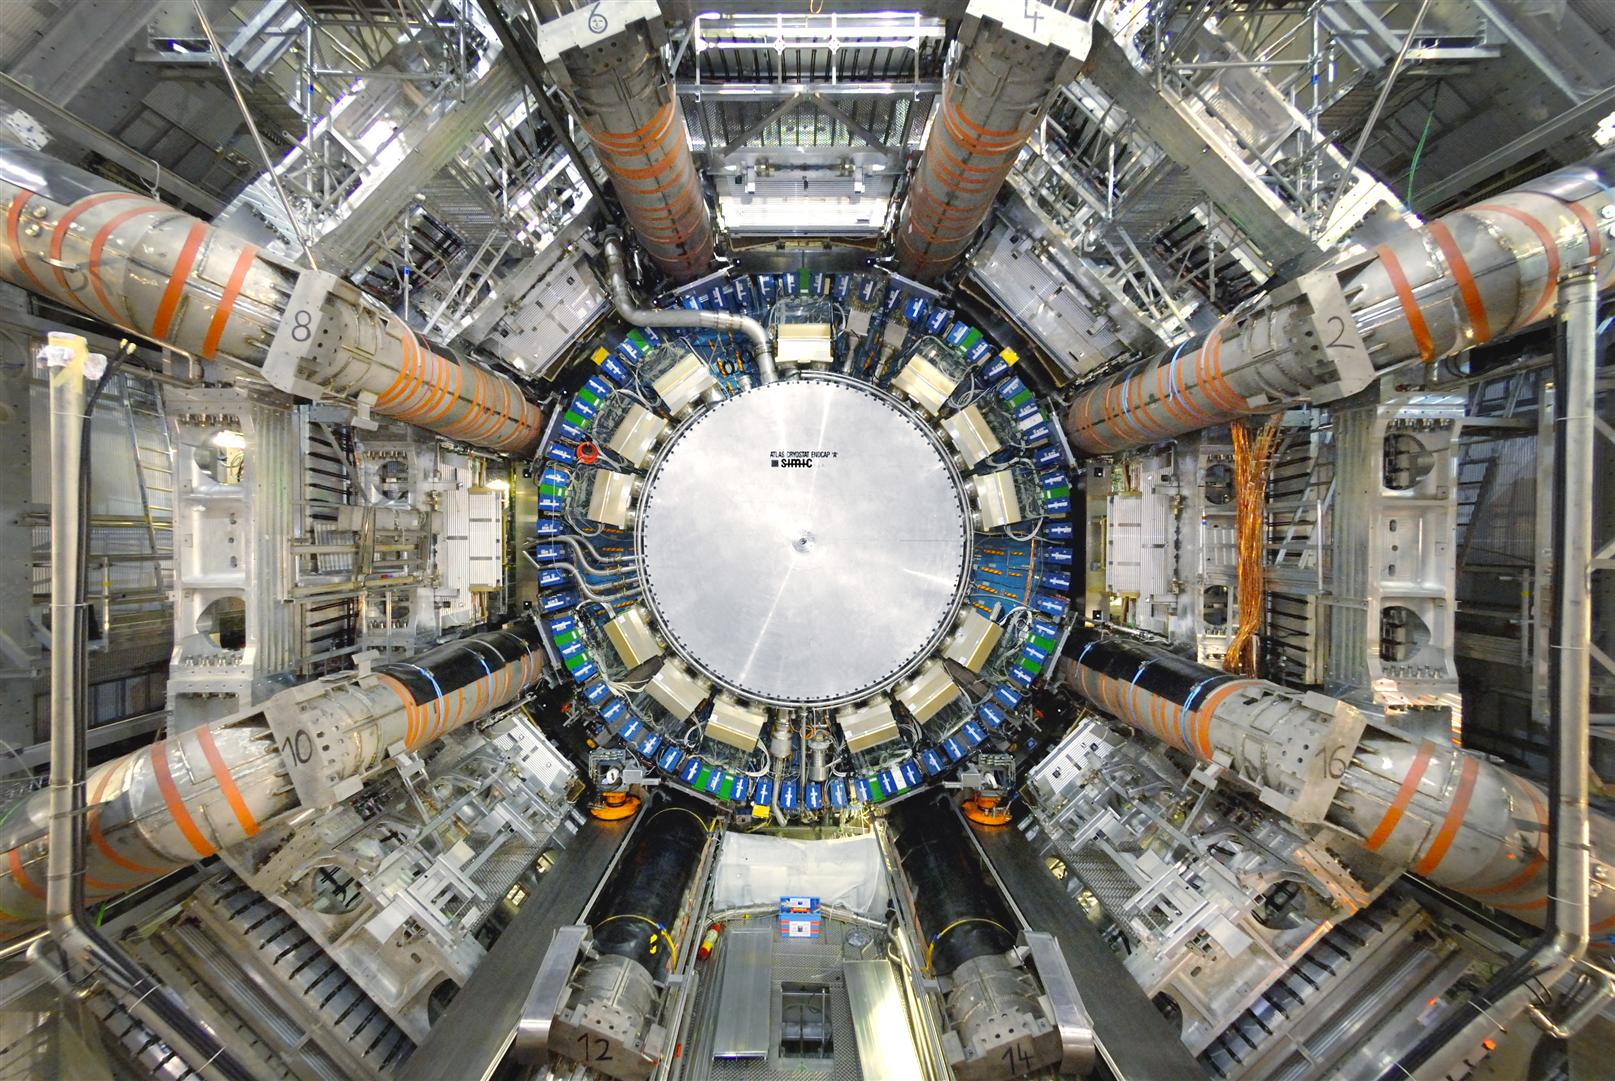
\includegraphics[width=0.5\textwidth]{atlas.jpeg}
\caption{The ATLAS detector at the Large Hadron Collider~\cite{atlas}.\label{fig:atlas}}
\end{figure}
